\subsection{Normal form of the same magnetic cantilever}
\label{sec:unified-normal-form}

In the dimensionless chart of Section~\ref{sec:unified-model}, write
\begin{equation}
 \begin{aligned}
 h_\star&=h_2+g(d^\top X),\\
 h_2&=\frac12\sum_{j=1}^n\nu_j(X_j^2+Y_j^2),\\
 g(z)&=1-\cos z-\frac{z^2}{2}.
 \end{aligned}
 \label{eq:beam-exact-h}
\end{equation}
The magnetic term in this expression is the complete analytic function.
In particular, its fourth-order part and its untruncated remainder are
\[
 \begin{aligned}
 h_{4,\star}&=-\frac{(d^\top X)^4}{24},\\
 T_{6,\star}&=1-\cos(d^\top X)-\frac{(d^\top X)^2}{2}\\
 &\quad+\frac{(d^\top X)^4}{24}.
 \end{aligned}
\]

\begin{proposition}[Magnetic twist and analytic tail]
\label{prop:magnetic-twist}
Let $I_j=(X_j^2+Y_j^2)/2$, and let $A_\star$ denote the Hessian with
respect to $I$ of the angular average of $h_{4,\star}$.
With $v=(d_1^2,\ldots,d_n^2)^\top$,
\begin{equation}
 \begin{aligned}
 (A_\star)_{jj}&=-\frac{d_j^4}{8},\\
 (A_\star)_{ij}&=-\frac{d_i^2d_j^2}{4}\quad(i\ne j),\\
 A_\star&=\frac{\operatorname{diag}(d_j^4)-2vv^\top}{8}.
 \end{aligned}
 \label{eq:beam-twist}
\end{equation}
and
\begin{equation}
 \det A_\star=(1-2n)8^{-n}\prod_{j=1}^n d_j^4.
 \label{eq:beam-twist-det}
\end{equation}
Thus every retained mode with nonzero tip-rotation participation contributes
to a nonsingular twist. For $n\geq2$, the twist has one negative and $n-1$
positive eigenvalues; positive definiteness is not required here.
If $D=\sum_j|d_j|$ and $\mathbb D_r^{2n}$ is a complex Cartesian polydisc,
then
\begin{equation}
 \|T_{6,\star}\|_r\leq\frac{(Dr)^6}{720}\cosh(Dr).
 \label{eq:beam-cos-tail}
\end{equation}
\end{proposition}

\begin{proof}
The angular averages are $\langle X_j^4\rangle=3I_j^2/2$ and
$\langle X_i^2X_j^2\rangle=I_iI_j$. All terms with an odd exponent in
some $X_j$ have zero average. Substitution gives~\eqref{eq:beam-twist}.
Factoring $\operatorname{diag}(d_j^2)$ on both sides gives a matrix
congruent to $(I_n-2\mathbf1\mathbf1^\top)/8$.
Its eigenvalues are $1/8$ with multiplicity $n-1$ and $(1-2n)/8$,
which proves the determinant and inertia statements.
For the analytic tail, expand the cosine and use
$(6+2k)!\geq6!(2k)!$ and $|d^\top X|\leq Dr$.
\end{proof}

For the two-mode, 32-element model, the magnetic-bias modes give
$\nu\simeq(1,6.152117504)$ and
$d\simeq(0.22567077,0.32179881)$.
Consequently $\det A_\star\simeq-1.303708\times10^{-6}$ and
$\sigma_{\min}(A_\star)\simeq5.8064\times10^{-4}$.
These quantities belong to the same cantilever model used for learning
and shape reconstruction.

\subsection{Complete learned Hamiltonian and transfer of twist}
\label{sec:unified-learning-twist}
The fitted family is
\begin{equation}
 h_\eta=h_2+\frac{b}{s_4}\,g(d^\top X)+\sum_{j=1}^{34}c_j\psi_j(X,Y),
 \label{eq:beam-learned-h}
\end{equation}
where $\eta=(b,c_1,\ldots,c_{34})$, $a=b/s_4$,
$s_4=\|q_\star\|_2$ is the fixed quartic coefficient normalizer and
the $\psi_j$ span the coefficient-space complement of the target
quartic direction. The class contains the complete target at
$\eta_\star=(s_4,0,\ldots,0)$; no cosine truncation error is assigned to the
training labels. The polynomial part is represented by matched real or
complex features. All bounds use the actually exported feature matrix,
so numerical orthogonality of its columns is not a proof assumption.

Let $F(z)=\bigl(g(d^\top X)/s_4,\psi_1(z),\ldots,\psi_{34}(z)\bigr)$,
and put $D(z)=[\nabla F_0(z),\ldots,\nabla F_{34}(z)]\in\mathbb R^{4\times35}$.
With $G_N=(4N)^{-1}\sum_i D(z_i)^\top D(z_i)$,
$\lambda_{\min}(G_N)\geq\underline\lambda>0$, empirical derivative
root-mean-square loss $r_N$ (averaged over all $4N$ scalar observations),
and a certified derivative-label error with the same root-mean-square
normalization bounded by $\epsilon_N$, the deterministic estimate is
\begin{equation}
 \|\eta-\eta_\star\|_2\leq
 b_N:=\frac{r_N+\epsilon_N}{\sqrt{\underline\lambda}}.
 \label{eq:beam-feature-bound}
\end{equation}
This estimate follows from the smallest singular value of the stacked
derivative design matrix and the triangle inequality.

The effective quartic coefficient vector is
$q_\eta=(b/s_4) q_\star+Uc$, where $U$ is the exported matrix of polynomial
features. Let $\mathcal A q$ be the symmetric twist matrix obtained by
angular averaging. Then the directly computable bound
\begin{equation}
 \begin{aligned}
 \|A_\eta-A_\star\|_2
 &\leq\|\mathcal A[q_\star/s_4\ U]\|_{2\to F}\,b_N\\
 &\quad+\delta_{A,\mathrm{dec}}<\sigma_{\min}(A_\star)
 \end{aligned}
 \label{eq:beam-twist-transfer}
\end{equation}
is sufficient for nonsingularity of the trained twist. The subscript $F$
denotes the Frobenius norm on symmetric matrices. In the two-mode raw
quartic basis, the previously derived bound
$\|\mathcal A\Delta q\|_2\leq\sqrt{19}\|\Delta q\|_2$
is also valid. A direct rational or interval check of $A_\eta$ can be
sharper than the sufficient loss-based bound.
Here $\delta_{A,\mathrm{dec}}$ bounds the exported decoder's rounding
error relative to its exact coefficient map; it is zero for exact
arithmetic and is explicitly included in the numerical certificate.
Specifically, the exported effective-quartic coefficient error
$\delta_{\mathrm{dec}}$ gives
$\delta_{A,\mathrm{dec}}=\sqrt{19}\delta_{\mathrm{dec}}$.

Define the finite-feature analytic bound by
\[
 \begin{aligned}
 B_F(r)^2&=\left(\frac{(Dr)^4}{24s_4}\cosh(Dr)\right)^2\\
 &\quad+r^8\sum_{j=1}^{34}\|\psi_j\|_{\mathrm{coeff},1}^2.
 \end{aligned}
\]
The same coefficient estimate gives a complete analytic perturbation bound,
\begin{equation}
 \|h_\eta-h_\star\|_r\leq b_N B_F(r)+\delta_{h,\mathrm{dec}}(r).
 \label{eq:beam-analytic-transfer}
\end{equation}
This controls the entire learned function on a complex domain, including
every higher-order magnetic term.

Suppose $\alpha_4=\min_{0<|k|_1\leq4}|k\cdot\nu|>0$.
The exact quartic Lie transformation associated with the full effective
$h_{4,\eta}$ gives
\[
 h_\eta\circ\Phi_\eta
 =\nu\cdot I+\tfrac12I^\top A_\eta I+\mathcal R_{6,\eta}.
\]
If $C_4,C_Z,C_\chi$ are the Cartesian coefficient norms of its quartic
part, angular average and homological generator, then
\begin{equation}
 \begin{aligned}
 \|\mathcal R_{6,\eta}\|_r
 &\leq512C_\chi(C_4+C_Z)r^6\\
 &\quad+\frac{|a|(2Dr)^6}{720}\cosh(2Dr).
 \end{aligned}
 \label{eq:beam-complete-normal-form-tail}
\end{equation}
This holds when $32C_\chi r^2<1$.
The first term is the exact quartic Lie remainder; the second bounds
$aT_{6,\star}\circ\Phi_\eta$ because the time-one flow maps the radius-$r$
polydisc into the radius-$2r$ polydisc. This identity retains the full
cosine rather than applying a theorem to an isolated quartic approximation.

With nonsingular $A_\eta$ and fourth-order nonresonance, the ordinary
Kolmogorov theorem applies on sufficiently small positive-action boxes
\citep[Theorems~A--B, arXiv:0908.2234v1]{poschel}.
Indeed, their action width is $O(r^2)$, their integrable Hessian is
$A_\eta$, and~\eqref{eq:beam-complete-normal-form-tail} is $O(r^6)$.
Choosing a Diophantine constant proportional to $r^2$ makes the analytic
KAM smallness quotient $O(r^2)$; reducing its proportionality constant
first leaves a positive-measure set of admissible frequencies.
This establishes local KAM families for the complete target and trained
cantilever Hamiltonians. The finite-amplitude result below is verified
separately by an a posteriori theorem and is not inferred from this
asymptotic statement.

\subsection{Validated invariant tori at finite physical amplitude}
\label{sec:unified-aposteriori}

The local normal-form argument can be supplemented by a finite-amplitude
certificate for the same complete Hamiltonian. We use the a posteriori
theorem of \citet{haro2019aposteriori}; the equation and table numbering
below refer to Theorem~3.1 and Appendix~B, Tables~1--3, of its archived
preprint, arXiv:1711.05515v1. The computation includes the analytic
interpolation error and uses ball arithmetic, rather than identifying a
small residual at finitely many sample points with an analytic norm.

The mathematical model certified here is specified exactly by the exported
binary coefficients. In particular,
\begin{equation}
 \begin{aligned}
 \nu&=\left(1,\frac{6926668524826847}{1125899906842624}\right),\\
 d&=\left(\frac{4065323231059343}{18014398509481984},
          \frac{2898505962069547}{9007199254740992}\right).
 \end{aligned}
 \label{eq:certified-beam-parameters}
\end{equation}
The target uses $a=1$ and zero quartic residual in
\eqref{eq:beam-learned-h}. Each trained case uses the exact dyadic value
of its exported cosine multiplier and every exported quartic coefficient.
This convention identifies the function being certified without hiding
floating-point parameter uncertainty. It establishes a result for the
exported two-mode reduction; independent finite-element and COMSOL
comparisons do not themselves prove an infinite-dimensional KAM theorem
for the continuum beam.

\begin{theorem}[Finite-amplitude tori of the target and trained models]
\label{thm:beam-finite-tori}
For the target Hamiltonian~\eqref{eq:beam-exact-h}, with parameters
\eqref{eq:certified-beam-parameters}, for each of the three primary exported
GC Hamiltonians with training seeds $17$, $43$, and $91$, and for the
additional seed-$17$ fit at noise amplitude $10^{-8}$, and for the
GC model fitted to independent COMSOL position--velocity trajectories,
there is a real
analytic, embedded Lagrangian torus $K_\infty:\mathbb T^2\to\mathbb R^4$
satisfying the invariance equation below, with the displayed frequency
for the first five models:
\begin{equation}
 \begin{aligned}
 X_h(K_\infty)&=DK_\infty\varpi,\\
 \varpi&=\frac{w_1}{2\pi}(1,\zeta),\\
 w_1&=\frac{49999589341}{50000000000}.
 \end{aligned}
 \label{eq:certified-invariance}
\end{equation}
where, with $\phi=(1+\sqrt5)/2$,
\begin{equation}
 \zeta=\frac{1876278\phi+592877}{304979\phi+96369}.
\label{eq:certified-quadratic-frequency}
\end{equation}
For the COMSOL-fitted model, the frequency is instead specified by
\begin{equation}
 \begin{aligned}
 w_1&=\frac{99999143141}{100000000000},\\
 \zeta&=\frac{974993\phi+427310}{158480\phi+69457}.
 \end{aligned}
 \label{eq:certified-comsol-frequency}
\end{equation}
It is chosen near that actual model's quartic normal-form frequency.
Angles have period one; $\varpi$ is measured in cycles per unit
dimensionless time. Each torus lies within $3\times10^{-41}$, in the
supremum norm on the complex strip of width $1/80$, of its computed
finite Fourier polynomial. The reconstructed beam has nonzero
millimetre-scale motion: the certified tip-displacement witness and the
bound valid for every point of the centerline are given in
Table~\ref{tab:finite-torus-certificate}.
\end{theorem}

\begin{proof}
We give the analytic estimates and specify the finite checks that close
them. Vector norms are maximum norms. Following the source convention,
analytic matrix norms are $\max_i\sum_j\sup_\theta|M_{ij}(\theta)|$,
with componentwise suprema on
$\mathbb T^2_\rho=\{\theta:|\operatorname{Im}\theta|_\infty<\rho\}$.
The phase-space domain is $\mathbb D_{3/10}^4$.

\emph{Frequency and the cohomological equation.}
The continued fraction of $\zeta$ has prefix
$[6;6,1,1,2,1,23,1,13,6,3]$ followed by an infinite tail of ones.
For the COMSOL-fitted model the prefix is
$[6;6,1,1,2,1,20,1,1,4,1,1,3,2]$, also followed by ones.
All partial quotients in either case are at most $23$.
The bounded-partial-quotient
inequality gives $|q\zeta-p|\geq1/(25|q|)$ for $q\ne0$.
As $w_1>9/10$ and $2\pi<7$, this implies
\begin{equation}
 |k\cdot\varpi|\geq\frac{\gamma}{|k|_1},\qquad
 \gamma=\frac9{1750},\qquad k\in\mathbb Z^2\setminus\{0\}.
 \label{eq:certified-dio}
\end{equation}
The case $k_2=0$ follows directly from $\varpi_1>9/70$.
We use the weaker exponent $\tau_K=3$ in the a posteriori theorem.
For a zero-mean analytic function $v$, Fourier division by
$2\pi i k\cdot\varpi$ and the count
$\#\{k:|k|_1=j\}=4j$ give, with $q=e^{-2\pi\delta}$,
\[
 \begin{aligned}
 \|\mathcal R_\varpi v\|_{\rho-\delta}
 &\leq\frac{2}{\pi\gamma}\frac{q(1+q)}{(1-q)^3}\|v\|_\rho\\
 &\leq\frac{e^{4\pi\rho}}{2\pi^4\gamma\delta^3}\|v\|_\rho
 <\frac{\|v\|_\rho}{\gamma\delta^3}.
 \end{aligned}
\]
These inequalities hold for $0<\delta<\rho=1/40$, so the
cohomological constant $c_R=1$ is justified directly.
Reconstructing the continued-fraction convergent matrix verifies the
stated frequency and Diophantine bound.

\emph{Global bounds and theorem constants.}
Write $h=h_2+a g(d^\top X)+p_4$, with quartic coefficient norm
$C_4=\sum_\alpha|(p_4)_\alpha|$.
The exact exported coefficients satisfy
$|a|\leq2$, $C_4<1/100$, $\|d\|_1<11/20$, and $\max\nu_j<7$.
The full cosine and its derivatives then give, on $\mathbb D_{3/10}^4$,
\begin{equation}
 \begin{aligned}
 c_{X_h,0}&=3,& c_{X_h,1}&=8,\\
 c_{X_h^\top,1}&=32,& c_{X_h,2}&=1.
 \end{aligned}
 \label{eq:HL-global-bounds}
\end{equation}
The third quantity bounds the derivative of the \emph{row-vector map}
$X_h^\top$. It bounds the sum of the absolute Jacobian entries and is
not the matrix norm of $(DX_h)^\top$.
For example, its linear part is $2(\nu_1+\nu_2)<28$; its remaining
bound is $2\|d\|_1^2(\cosh(3\|d\|_1/10)-1)+12C_4(3/10)^2<1$.
For the second derivative, the row-sum tensor estimate
$2\|d\|_1^3\sinh(3\|d\|_1/10)+24C_4(3/10)<1$ suffices.
All geometric tensors are constant canonical tensors with norm one
and zero derivatives.

Let $J=\left(\begin{smallmatrix}0&I\\-I&0\end{smallmatrix}\right)$,
$L=DK$, $B=(L^\top L)^{-1}$, and $N=-JLB$.
In the source convention the symplectic matrix is $\Omega=-J$.
The torsion used in the theorem is therefore
\begin{equation}
 T=-N^\top J\bigl(DX_h(K)N-D_\varpi N\bigr).
 \label{eq:HL-torsion}
\end{equation}
There are no additional first integrals ($n=d=2$, canonical Case~III).
Choose $\rho=1/40$, $\rho_\infty=1/80$, $a_1=a_2=2$, $a_3=12$,
$\delta=\rho/12$, and the iteration parameter $\nu_{\rm it}=1$.
The bounds used with strict margins are
\[
 \begin{aligned}
 \|DK\|_\rho&<1<\sigma_K=2,\\
 \|DK^\top\|_\rho&<\tfrac32<\sigma_{K^\top}=2,\\
 \|B\|_\rho&<3<\sigma_B=4,
 \end{aligned}
\]
\[
 \|\langle T\rangle^{-1}\|<10^5<\sigma_T=2\times10^5,
 \qquad \|K\|_\rho<\tfrac15.
\]
The last inequality leaves a phase-space distance margin $1/10$.
Substitution in Tables~1--3 gives exact rational constants with the
following decimal approximations:
\begin{equation}
 \begin{aligned}
 C_1&\simeq4.843521623\times10^{46},\\
 C_2&\simeq4.940319879\times10^{21},\\
 \frac{\gamma^4\rho^{12}}{C_1}&>8.6086\times10^{-76}.
 \end{aligned}
 \label{eq:HL-evaluated-constants}
\end{equation}
The rational recurrence in those tables is evaluated using rational or
ball arithmetic; rounded decimal values are used only for display. The
source's $C_{\rm sym}$ follows from the Case~III block identity in
Remark~4.7, immediately after Eq.~(4.39):
$C_{\rm sym}=\max\{1,\sigma_B^2\}C_{\Omega_L}=192$,
using $\sigma_B=4$ and $C_{\Omega_L}=12$.
This uses $C_{\Omega_L}$ from the geometric identity in place of the
$C_{\widetilde\Omega_L}$ printed in the corresponding row of Table~1.

\emph{Analytic residual and torsion checks.}
For each case the approximate embedding $K$ is an exact dyadic finite
Fourier polynomial supported on $|k_j|\leq63$.
Conjugate symmetry is checked exactly.
Its derivative and wide-strip norms are bounded by
$\sum_k|K_k|e^{2\pi s|k|_1}$ and the corresponding differentiated sums.
To bound $B$, compare $K$ with
$K_0=(\frac1{10}\cos2\pi\theta_1,
\frac1{10}\cos2\pi\theta_2,-\frac1{10}\sin2\pi\theta_1,
-\frac1{10}\sin2\pi\theta_2)$.
Put $e_L=\|D(K-K_0)\|$ and $e_{L^\top}=\|D(K-K_0)^\top\|$.
As $DK_0^\top DK_0=(2\pi/10)^2I$ exactly, the checked inequality
\[
 \begin{aligned}
 &\|DK_0^\top\|e_L+e_{L^\top}\|DK_0\|\\
 &\qquad+e_{L^\top}e_L<(2\pi/10)^2
 \end{aligned}
\]
provides a Neumann-series inverse bound for the analytic Gram matrix.

The residual $E=X_h(K)-DK\varpi$ is evaluated with 512-bit Arb balls
on a $256\times256$ grid, including ball sine evaluations and all
quartic terms. Let $\mathcal I_mE$ be its trigonometric interpolant,
$\widehat\rho=1/4$, and $M\geq\|E\|_{\widehat\rho}$, computed directly
from the finite Fourier polynomial and the entire Hamiltonian.
Fourier decay, the two-dimensional union bound for the omitted modes,
and the alias sum give
\begin{equation}
 \begin{aligned}
 \|E\|_\rho&\leq\|\mathcal I_mE\|_\rho+E_{\rm tail},\\
 E_{\rm tail}&=8M\frac{1+q}{(1-q)^2}e^{-\pi(\widehat\rho-\rho)m}.
 \end{aligned}
 \label{eq:HL-alias-bound}
\end{equation}
Here $q=e^{-2\pi(\widehat\rho-\rho)}$ and $m=256$.
Both the omitted Fourier tail and the aliased coefficients are included
in the factor $8$. The larger strip is used only to estimate the
composition residual; the entire full-cosine Hamiltonian is defined
there even when $K(\mathbb T^2_{\widehat\rho})$ leaves the smaller
phase-space domain used by the KAM iteration.

For the mean torsion, the same Gram estimate on the strip $7/100$
proves $\|N\|,\|N^\top\|<6$. Since $\|\varpi\|_1<2$, Cauchy's
inequality on the strip $6/100$ gives $\|D_\varpi N\|<1200$, and hence
$\|T\|<6(8\cdot6+1200)<10^4$.
An Arb trapezoidal average on $128^2$ nodes is corrected by
\[
 10^4\left[\left(\frac{1+z}{1-z}\right)^2-1\right],
 \qquad z=e^{-2\pi(6/100)128}.
\]
The derivative of $B$ in this evaluation is calculated by differentiating
its inverse identity, so no differentiated interpolation of $N$ is used.
Inverting the resulting interval $2\times2$ matrix proves the stated
bound on $\langle T\rangle^{-1}$.

The resulting bounds in Table~\ref{tab:finite-torus-certificate} satisfy
\begin{equation}
 \frac{C_1\|E\|_\rho}{\gamma^4\rho^{12}}<1.
 \label{eq:HL-final-smallness}
\end{equation}
The cited theorem supplies the invariant Lagrangian torus and
$\|K_\infty-K\|_{\rho_\infty}
\leq C_2\|E\|_\rho/(\gamma^2\rho^6)<3\times10^{-41}$.
For completeness, embeddedness can also be checked quantitatively:
writing $X_j-iY_j=0.1e^{2\pi i\theta_j}+\xi_j$, the verified
$C^0$ and $C^1$ differences from $K_0$ make the phase map a
degree-one map with derivative less than $1/2$ from the identity.
It is a diffeomorphism. The same inequality holds after adding the
KAM correction and its Cauchy derivative bound on a smaller strip.

\emph{Physical displacement.}
The exact exported shape matrix maps $X$ to the Hermite nodal
displacements and slopes. On an element of length $\ell$, the cubic
Bernstein control values are
$w_0$, $w_0+\ell\vartheta_0/3$,
$w_1-\ell\vartheta_1/3$, and $w_1$.
For a control row $b$, its value on the invariant torus is bounded by
$\sum_{j=1}^2|b_j|(\sum_k|(X_j)_k|+3\times10^{-41})$.
The convex-hull property therefore bounds every centerline point,
every phase, and all time. A ball evaluation at phase $(0,0)$ gives
the separate positive lower witness in the table. These bounds use
the same exported shape map as the learning and beam reconstruction.
\end{proof}

\begin{table*}[t]
\centering\small
\caption{Finite-amplitude certificates for the complete target and actual
trained Hamiltonians. Displayed bounds are rounded outward. The lower
witness is tip displacement at one phase; the upper bound covers the
entire reconstructed centerline at all phases.}
\label{tab:finite-torus-certificate}
\begin{tabular}{lrrrr}
\hline
Model & $\|E\|_\rho$ upper & KAM quotient upper &
Tip lower (mm) & Centerline upper (mm)\\
\hline
Target & $2.7310\,10^{-77}$ & $0.031724$ & $1.8977905$ & $1.8977964$\\
GC17 & $2.7372\,10^{-77}$ & $0.031796$ & $1.8927460$ & $1.8927517$\\
GC43 & $2.7538\,10^{-77}$ & $0.031988$ & $1.8837514$ & $1.8837573$\\
GC91 & $2.7285\,10^{-77}$ & $0.031694$ & $1.9077295$ & $1.9077354$\\
GC17 ($10^{-8}$ noise) & $2.7311\,10^{-77}$ & $0.031724$ & $1.8977399$ & $1.8977457$\\
GC (COMSOL states) & $2.7330\,10^{-77}$ & $0.031746$ & $1.8977374$ & $1.8977433$\\
\hline
\end{tabular}
\end{table*}

\begin{figure*}[t]
\centering
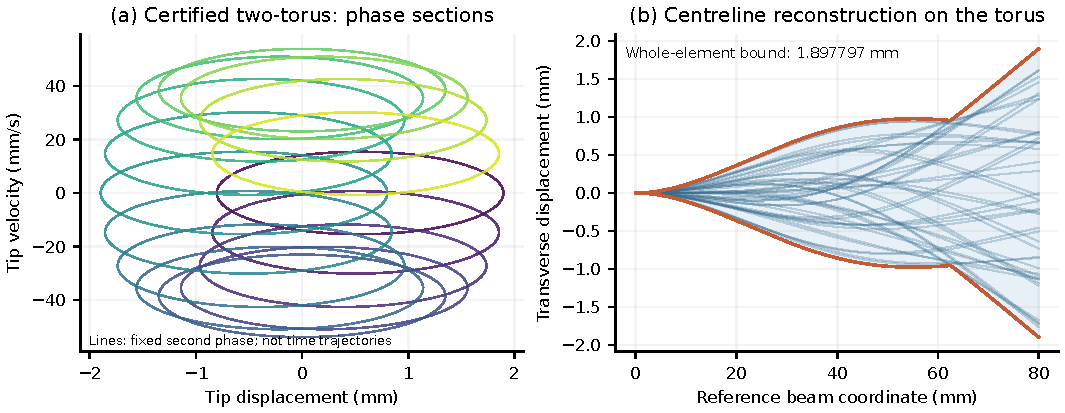
\includegraphics[width=\textwidth]{figures/fig_certified_torus_geometry.pdf}
\caption{The certified target torus in the same SI beam coordinates.
(a) Tip displacement and velocity along sampled sections with the second
phase fixed; these curves are not time trajectories.
(b) Sampled centerlines and a plotted phase envelope.
The separate whole-element Bernstein/Fourier certificate bounds every
centerline point on the corrected invariant torus by $1.897797$ mm.
Sampling illustrates the geometry; the analytic certificate supplies
the all-phase bound.}
\label{fig:certified-torus-geometry}
\end{figure*}

The additional low-noise fit connects the two certificates on one actual
learned Hamiltonian. Its nonzero derivative MSE is
$3.3866649\times10^{-17}$. The outward Gram lower bound
$6.0167\times10^{-8}$, together with the label and decoder error budgets,
gives a twist-error upper bound $2.81119\times10^{-4}$, smaller than
the target singular-value lower bound $3.03081\times10^{-4}$.
The fifth row of the table uses these same fitted coefficients. Thus
the nonzero-loss twist certificate and the finite-amplitude
KAM certificate concern the same fitted function; the latter additionally
uses the full analytic invariance residual, as required by the theorem.

The sixth row certifies the actual GC function obtained from four
independent COMSOL position--velocity trajectories by integral matching.
The fit uses state increments and feature integrals, without reconstructed
acceleration labels. Its exported cosine multiplier is
$a=1.022324882191665$; every exported quartic term is included in
the analytic verification, using the fitted coefficients without
re-estimation. The frequency in~\eqref{eq:certified-comsol-frequency}
admits the same conservative
$\gamma=9/1750$, so the global bounds and theorem constants above
remain unchanged. In this case the checked inverse averaged torsion
is below $94762$, within the required $10^5$ margin.

This result certifies one specified nonresonant torus in each Hamiltonian
at a useful physical amplitude. It does not attach a measured phase-space
volume to these individual tori. Positive-measure families near the elliptic
equilibrium follow from the separate normal-form argument above;
the finite-amplitude theorem and the energy-based safety theorem have
distinct hypotheses and conclusions.

\subsection{Positive-measure families around the certified tori}
\label{sec:certified-torus-families}

The nondegeneracy retained by the a posteriori iteration gives a further
conclusion at the same finite-amplitude motion.

\begin{corollary}[KAM stability of the certified finite-amplitude tori]
\label{cor:finite-torus-families}
Each of the six tori in Theorem~\ref{thm:beam-finite-tori}, and the
additional integral-COMSOL torus in
Section~\ref{sec:validated-integral-learning}, is accumulated by
positive-measure families of analytic Lagrangian invariant tori.
In analytic symplectic tubular coordinates $(\theta,I)$ centered on that
torus, their relative Lebesgue measure in
$\mathbb T^2\times\{|I|_\infty<r\}$ tends to one as $r\to0$.
This is an asymptotic statement about neighborhoods of the certified
millimetre-amplitude torus; it does not specify a numerical tube
thickness or a percentage in a preassigned experimental domain.
In particular, for any prescribed fraction $p<1$, a sufficiently thin
tube has relative invariant-torus measure greater than $p$. The present
statement is existential in the tube radius.
\end{corollary}

\begin{proof}
The inequalities controlling the inverse averaged torsion in the
Haro--Luque iteration are uniform at every step: see their
Eqs.~(5.65)--(5.67) and the summation in Section~5.3.
The strict margin used in~\eqref{eq:HL-evaluated-constants} therefore gives
\[
 \|\langle T_\infty\rangle^{-1}\|\leq2\times10^5.
\]
This is nondegeneracy of the final invariant object, not only of its
numerical approximation.

An analytic Lagrangian neighborhood chart $\Psi$ can be chosen with
$\Psi(\theta,0)=K_\infty(\theta)$ and first derivative
$D\Psi(\theta,0)=[L_\infty,N_\infty]$.
One construction starts with $K_\infty(\theta)+N_\infty(\theta)I$ and
uses the relative analytic Moser correction. The forms agree on the
zero section; the relative primitive and its correcting vector field
are $O(|I|^2)$, so the correction preserves this first jet.
In these coordinates invariance implies
\begin{equation}
 \begin{aligned}
 h\circ\Psi&=e+\varpi\cdot I+\tfrac12 I^\top A(\theta)I\\
 &\quad+O(|I|^3).
 \end{aligned}
 \label{eq:torus-tubular-hamiltonian}
\end{equation}
The automatic-reducibility identity of Haro--Luque Section~2.4 is
\[
 \begin{aligned}
 &DX_h(K_\infty)P-D_\varpi P\\
 &\qquad=P\begin{pmatrix}0&T_\infty\\0&0\end{pmatrix},
 \end{aligned}
\]
where $P=[L_\infty,N_\infty]$.
Comparing this with the linearized vector field of
\eqref{eq:torus-tubular-hamiltonian} gives $A=T_\infty$.
More generally, changing the symplectic normal frame to
$N_\infty+L_\infty S(\theta)$, with $S$ symmetric, changes this block
to $T_\infty-D_\varpi S$, whose average is the same.
Hence $\overline A=\langle A\rangle$ is nonsingular independently of
this choice of normal frame.

The quadratic normal form is justified without a formal-series
convergence assumption. Solve the matrix homological equation
$D_\varpi S=A-\overline A$ with zero average by
\[
 S_k=\frac{A_k}{2\pi i k\cdot\varpi}\quad(k\ne0),\qquad S_0=0.
\]
Equation~\eqref{eq:certified-dio} and analyticity make this series
convergent on every strictly smaller angle strip; the cohomological
bound established above controls it there.
The exact time-one Hamiltonian flow of
$\chi_2(\theta,I)=\tfrac12 I^\top S(\theta)I$ exists on a sufficiently
thin tube and fixes $I=0$. With the pullback convention
$L_{\chi}F=\{F,\chi\}$, it changes the quadratic coefficient to
$\overline A$ and leaves an analytic $O(|I|^3)$ remainder.
The resulting normal form satisfies the hypotheses of
\citet[Theorem~6, analytic case]{bounemoura2016torus}:
the frequency is nonresonant, the averaged quadratic form is
nonsingular, and the full remainder is analytic. That theorem gives
the claimed density-one families. Symplectic coordinate changes
preserve volume, and the constant factor relating the dimensionless
chart to SI canonical coordinates cancels in relative measure.
\end{proof}

This corollary establishes the local abundance of invariant tori around
the certified motion. Section~\ref{sec:measure-definition} defines their
relative measure on a specified phase-space domain. For the
integral-COMSOL fit, Appendix~\ref{app:measure-proof} supplements the local
result with an explicit symplectic chart, a complete analytic remainder
and a conservative quantitative bound on a fixed tube. The tube width
and the resulting measure bound are reported together to distinguish
this rigorous local estimate from the wider numerical sampling domain.
